\section{Methods}
\label{sec:methods}

\subsection{Gravity-aligned odometry bridge}
\label{sec:bridge}

FAST-LIO2~\cite{xu2022fastlio2} (or Leg-KILO~\cite{ou2024legkilo}) estimates
$\T{ci}{body}(t) \in \SE{3}$ with the world frame \frm{camera\_init} equal to the IMU frame at
start. If the robot starts tilted by $\theta$, that world is tilted: a horizontal distance $s$
appears as a height change and a shorter planar distance,
\begin{equation}
  \Delta z \approx s \sin\theta, \qquad \frac{\Delta s_{xy}}{s} = 1 - \cos\theta ,
  \label{eq:tilt}
\end{equation}
i.e.\ 3.5, 8.7 and 13.9~cm of false height per metre for $\theta = 2^\circ, 5^\circ,
8^\circ$. Mapping and perception filter obstacles in a height band above the floor and
assume a level frame, so a start at the previous 8° limit puts the floor 5~m ahead 0.7~m above
the band. Two measures remove this. A launch prefix holds the estimator (and every respawn)
until the IMU is still and level: largest angular rate below 0.03~rad/s, relative standard
deviation of $\|\vect{f}\|$ below 1\,\%, tilt at most 3°. Then localization measures the mean
specific force $\bar{\vect{f}}$ over a still window and computes the up direction of the base at
start, $\vect{u} = \mathbf{R}^{\mathrm{base}}_{\mathrm{imu}}\, \mathbf{R}^{\mathrm{ci}}_{
\mathrm{body}}(t)\, \bar{\vect{f}} / \|\cdot\|$. The level rotation $L$ is the rotation that
aligns $\vect{u}$ with $\vect{z}$, with its yaw removed so that \frm{odom}'s $x$ axis keeps the
start heading. The bridge publishes
\begin{equation}
  \T{odom}{ci} = L\, \T{base}{imu}, \qquad \T{body}{base} = \big(\T{base}{imu}\big)^{-1},
\end{equation}
so $\T{odom}{base}(t_0) = L$: \frm{odom} starts at \frm{base\_link}, with $z$ against gravity.
After an estimator restart it is levelled again. Only the direction of $\bar{\vect{f}}$ is used,
so accelerometer units do not matter.

The odometry monitor compares the estimator speed with the robot's own odometry as a residual
test~\cite{page1954cusum}:
\begin{equation}
  \begin{aligned}
    r_k &= v^{\mathrm{lio}}_k - v^{\mathrm{leg}}_k, \qquad
    \chi^2_k = \frac{r_k^2}{\sigma_{\mathrm{lio}}^2 + \sigma_{\mathrm{leg}}^2},\\
    S_k &= \max\big(0,\ S_{k-1} + \chi^2_k - \kappa\big),
  \end{aligned}
  \label{eq:cusum}
\end{equation}
with an alarm while $S_k > h$ ($\kappa = 3.84$, the 95\,\% quantile of $\chi^2_1$, $h = 20$).
The thresholds follow from the sensor variances, not from robot speeds. A restart is detected
only when the pose returns to the origin after a message gap or a physically impossible
translation jump; a yaw change alone (turning in place near the start) never counts.

\subsection{Fiducial-anchored SE(2) EKF}
\label{sec:loc}

\begin{figure}[t]
  \centering
  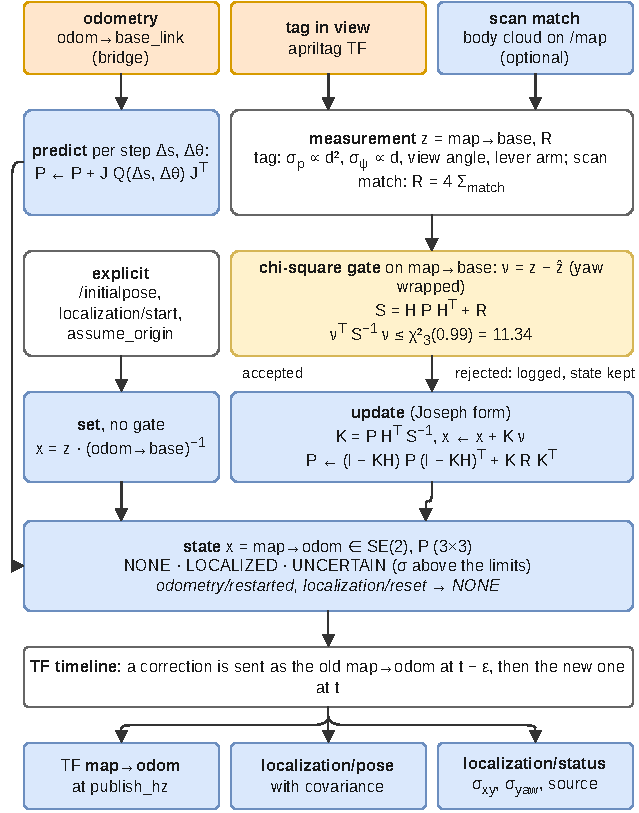
\includegraphics[width=\columnwidth]{localization_ekf}
  \caption{Localization: an EKF over \frm{map}$\to$\frm{odom}, predicted by odometry motion and
    corrected by fiducials, scan matching and explicit operator input.}
  \label{fig:ekf}
\end{figure}

The original stack replaced \frm{map}$\to$\frm{odom} by every tag detection, without
uncertainty and with ad-hoc rejection thresholds (0.5~m, 15°) that compared the correction
itself. A heading error $\delta\psi$ of that correction displaces the robot by
$e_\perp \approx L\,\delta\psi$ after a distance $L$ from the tag (17.5~cm after 10~m at
$\delta\psi = 1^\circ$), and a small rotation of \frm{map}$\to$\frm{odom} far from the odometry
origin moves the robot metres. Dharma estimates the correction itself (Fig.~\ref{fig:ekf}).

\textbf{State and prediction.} The state is $\vect{x} = (x, y, \psi)$ of $\T{map}{odom}$ with a
$3\times3$ covariance $\mathbf{P}$. With the odometry pose $\vect{o} = \T{odom}{base}$, the
robot pose is $h(\vect{x}) = \vect{x} \oplus \vect{o}$ and its Jacobian with respect to the state
\begin{equation}
  \mathbf{H} = \begin{bmatrix} 1 & 0 & -(y_b - y) \\ 0 & 1 & x_b - x \\ 0 & 0 & 1 \end{bmatrix}
\end{equation}
contains the lever arm from the \frm{odom} origin to the robot $(x_b, y_b)$. Drift is
proportional to motion: the odometry is counted in steps of distance $\Delta s$ and rotation
$\Delta\theta$, and
\begin{equation}
  \begin{aligned}
    \mathbf{P} &\leftarrow \mathbf{P} + \mathbf{H}^{-1} \mathbf{Q} \mathbf{H}^{-\top},\\
    \mathbf{Q} &= \mathrm{diag}\big(\sigma_{s}^2 \Delta s,\ \sigma_{s}^2 \Delta s,\
    \sigma_{\psi s}^2 \Delta s + \sigma_{\psi\theta}^2 \Delta\theta\big),
  \end{aligned}
\end{equation}
so a robot standing still never becomes uncertain (defaults $\sigma_s = 0.03$~m$/\sqrt{\mathrm{m}}$,
$\sigma_{\psi s} = 0.1^\circ/\sqrt{\mathrm{m}}$, $\sigma_{\psi\theta} = 0.5^\circ/\sqrt{
\mathrm{rad}}$).

\textbf{Update and gate.} A source measures the robot pose $\vect{z}$ of \frm{map}$\to$
\frm{base\_link} with covariance $\mathbf{R}$. The innovation is taken on the robot pose,
\begin{equation}
  \begin{aligned}
    \vect{\nu} &= \vect{z} - h(\vect{x}), \qquad \mathbf{S} = \mathbf{H}\mathbf{P}\mathbf{H}^\top
    + \mathbf{R},\\
    d^2 &= \vect{\nu}^\top \mathbf{S}^{-1} \vect{\nu} \le \chi^2_{3,0.99} = 11.34,
  \end{aligned}
  \label{eq:gate}
\end{equation}
(yaw wrapped), so a fix is judged by how far it moves the robot. The gate grows with
$\mathbf{P}$ after a long drive and is tight right after a correction. Accepted measurements
update the state with $\mathbf{K} = \mathbf{P}\mathbf{H}^\top\mathbf{S}^{-1}$ and the
Joseph-form covariance $\mathbf{P} \leftarrow (\mathbf{I}-\mathbf{K}\mathbf{H})\mathbf{P}
(\mathbf{I}-\mathbf{K}\mathbf{H})^\top + \mathbf{K}\mathbf{R}\mathbf{K}^\top$, with a floor on
the robot pose covariance against overconfidence. The state is \textsc{none} before the first
fix and \textsc{uncertain} when $\sigma_{xy}$ or $\sigma_\psi$ exceed their limits.

\textbf{Sources.} A tag with known map pose $\T{map}{tag}$ seen at $\T{cam}{tag}$ gives
\begin{equation}
  \T{map}{base} = \T{map}{tag} \big(\T{base}{cam}\, \T{cam}{tag}\big)^{-1},
\end{equation}
computed in SE(3) (the optical frame is never planar) and flattened to SE(2). Its noise grows
with distance $d$ and view angle $\alpha$, $\sigma_p = \sigma_1 d^2/\cos\alpha$,
$\sigma_\psi = \sigma_{\psi1} d/\cos\alpha$, and a heading error moves the robot around the tag:
with $\vect{l}$ the robot-to-tag vector rotated by 90°, $\mathbf{R}_{xy} = \sigma_p^2\mathbf{I} +
\sigma_\psi^2\vect{l}\vect{l}^\top$ and $\mathbf{R}_{xy,\psi} = \sigma_\psi^2\vect{l}$, so far
tags count little. Optional scan matching projects the registered cloud into the level frame,
keeps a height band and matches it on the map with a correlative matcher~\cite{olson2009csm},
using the scaled covariance of the score surface. Operator pose estimates, an explicit
\texttt{localization/start} and \texttt{assume\_origin} set the state without gate, so a far
but consistent tag after a kidnapping still relocalizes on request.

\textbf{Publication.} tf2 interpolates between samples, so a correction between two periodic
samples would map scans to poses that never existed. A correction is therefore published as
the previous \frm{map}$\to$\frm{odom} at $t-\epsilon$ ($\epsilon = 1$~ms) and the new value at
$t$. The robot pose is also published with its covariance $\mathbf{H}\mathbf{P}\mathbf{H}^\top$.

\subsection{Occupancy mapping with jump and correction gating}
\label{sec:map}

Each cell holds log-odds $l = \log\frac{p}{1-p}$ updated by
\begin{equation}
  l_t = \mathrm{clip}\big(l_{t-1} + \{l_{\mathrm{hit}} = 0.85,\ l_{\mathrm{miss}} = -0.4\},\
  [-2, 3.5]\big),
\end{equation}
occupied above $\mathrm{logit}(0.65) = 0.619$; free space is carved only up to the nearest hit
per angular bin, so glass and open doors are not cleared. A saturated cell needs
$\lceil (3.5 + 0.619)/0.4 \rceil = 11$ crossing rays to become free. Points are kept between a
minimum and maximum height above the floor (the base height below \frm{base\_link}), measured in
the levelled map frame. Since scans are integrated at their TF pose, the map is only as good as
the pose; two gates keep bad poses out. A scan whose sensor moved more than
$d_{\max} + v_{\max}\Delta t$ (or turned more than $\psi_{\max} + \omega_{\max}\Delta t$) since
the previous scan holds integration until a scan agrees with the map again, and a scan during
which \frm{map}$\to$\frm{odom} changed (a correction in flight) is skipped. The grid side is
capped. An optional refinement matches each scan on the current grid before integrating it;
loop closure is future work.

\subsection{Footprint-aware planning}
\label{sec:plan}

The planning costmap is built from the map with radii from the profile: a cell closer than
$r_{\mathrm{lethal}} = r_{\mathrm{in}} + m$ to an obstacle is lethal for every heading; up to
$r_{\mathrm{c}} + m$ a collision depends on the heading and the planner checks the
\emph{oriented} footprint at the heading the follower will use; beyond, the cost decays to 1 at
the inflation radius $R$,
\begin{equation}
  c(d) = 1 + W\, \frac{e^{-k(d - r_{\ell})} - e^{-k(R - r_{\ell})}}
  {1 - e^{-k(R - r_{\ell})}}, \qquad r_{\ell} < d < R,
\end{equation}
with $r_\ell = r_{\mathrm{lethal}}$ and $W = 5$. A*~\cite{hart1968astar} runs 8-connected without corner cutting and with the
octile heuristic (admissible since $c \ge 1$). Line-of-sight shortcuts are accepted only when
they stay as far from walls as the search (a line touching a cell corner counts both side
cells, so it never slips through a diagonal pinch); smoothing is discarded when it touches a
lethal cell. Where the footprint check fails along the result, the offending cells are blocked
and the search repeats.

\subsection{Path tracking, speed profile and path shift}
\label{sec:track}

All speed limits use one braking model: the distance to stop from speed $v$ with reaction time
$\tr$ and deceleration $a$, and its inverse, the highest speed that stops within a room $d$,
\begin{equation}
  D(v) = v\,\tr + \frac{v^2}{2a}, \qquad
  v^*(d) = a\Big(-\tr + \sqrt{\tr^2 + 2d/a}\Big).
  \label{eq:braking}
\end{equation}
The speed profile along the route takes the curvature limit $v_i \le \sqrt{a_{\mathrm{lat}}
/|\kappa_i|}$, the approach speed at stop points and the end, a backward pass
$v_i \le \sqrt{v_{i+1}^2 + 2 a_{\mathrm{dec}} \Delta s_i}$, the braking model \eqref{eq:braking}
before every stop and a forward pass $v_{i+1} \le \sqrt{v_i^2 + 2 a_{\mathrm{acc}} \Delta s_i}$.
The default holonomic controller steers toward a carrot a distance $L$ ahead on the route, so
the cross-track error decays as $e(t) = e_0 e^{-t v/L}$ (95\,\% after $3L$ of travel,
independent of speed) and the heading is controlled separately toward the route direction; five
other controllers (pure pursuit~\cite{coulter1992purepursuit}, PID, LQR,
Stanley~\cite{thrun2006stanley}, MPPI~\cite{williams2017mppi}) are plugins. Reactive avoidance
outputs a heading offset (rad, a rotation of the direction of travel) and a yaw-rate bias
(rad/s), applied the same way by every controller; the original single \emph{steering bias}
was a rate in the message and an angle in one controller.

\textbf{Path shift.} For omnidirectional robots, obstacles of the 360° safety scan are expressed
in route coordinates $(s, d)$~\cite{werling2010frenet}. A lateral offset $o$ is clear when no
point lies in the corridor $|d - o| < w + c$ ($w$ the half width, $c$ a clearance) from the rear edge of the body to a look-ahead
$\ell$ beyond its front edge. The offset is
\begin{equation}
  o^* = \arg\min_{o\ \mathrm{clear}} |o| + \lambda |o - o_{\mathrm{prev}}|,
  \label{eq:shift}
\end{equation}
with hysteresis and a delay before returning toward the route. Without a clear offset the
robot keeps the one with the largest free distance. The speed limit is $v^*(d_{\mathrm{free}} -
m)$ with $d_{\mathrm{free}}$ the smallest free distance over the target offset, the commanded
offset and the measured lateral offset, so a robot still sliding sideways is not sped up by the
offset it has not reached. Near a stop point the robot stays on the route and waits.

\subsection{Protective field and fail-safe sensing}
\label{sec:field}

\begin{figure*}[t]
  \centering
  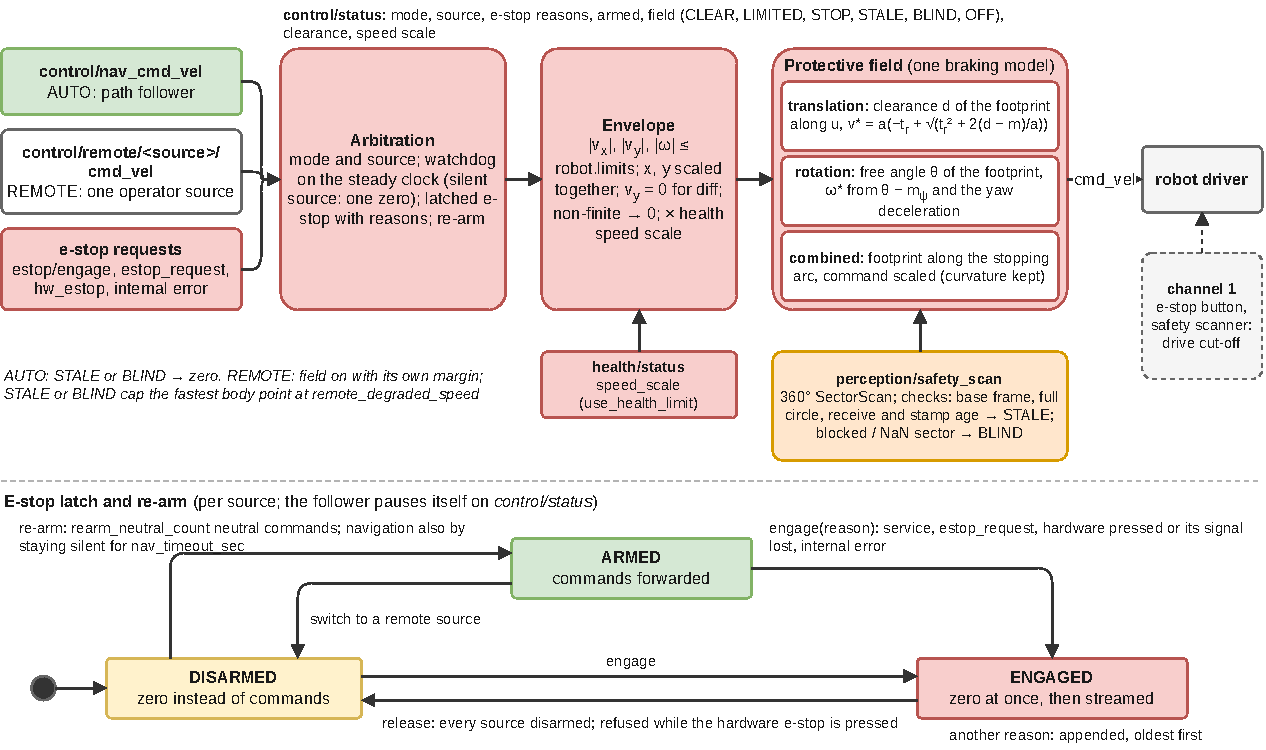
\includegraphics[width=0.9\textwidth]{safety_pipeline}
  \caption{Safety layer: arbitration, envelope and protective field in front of the robot's
    \topic{cmd\_vel}, and the e-stop latch with re-arm. Channel 1 (hardware) cuts the drive
    independently of any software.}
  \label{fig:safety}
\end{figure*}

The control multiplexer (Fig.~\ref{fig:safety}) arbitrates navigation (AUTO) and one operator
source (REMOTE) with watchdogs on the steady clock, clamps every command to the robot's
envelope (non-finite values become zero) and limits it with a protective field on the 360°
safety scan, a form of speed and separation monitoring~\cite{isots15066,marvel2016ssm}.

\textbf{Translation.} For the direction $\hat{\vect{u}}$ of the commanded translation, the
clearance $d_t$ is the distance the footprint can move before touching a scan point (points
ahead of the leading edge within the body corridor widened by a lateral margin, and zero for a
point beside or inside the body). The speed is scaled to $v^*(d_t - m)$, keeping the direction.

\textbf{Rotation.} Turning in place, the corners sweep the ring $r_{\mathrm{in}} < r \le
r_{\mathrm{c}}$ (0.28 to 0.49~m for the default profile), which the original field ignored. The
free angle $\theta_f$ is found by rotating the ring points in 1° steps until one enters the
footprint, and $|\omega| \le \omega^*(\theta_f - m_\psi)$ with the same model and the yaw
deceleration.

\textbf{Combined motion.} For a twist $(v_x, v_y, \omega)$ the robot keeps the command for
$\tr$ and then brakes both axes proportionally over $T_b = \max(v/a, |\omega|/\alpha)$; it
covers the constant-twist arc up to the parameter $u = \tr + T_b/2$ (exactly $D(v)$ on a
straight line). The footprint is checked at poses along the arc; if the first contact is at
$u_c$, scaling the command by $s$ keeps the curvature and covers $s\tr + s^2 T_b/2$, so the
largest clear scale is
\begin{equation}
  s = \frac{-\tr + \sqrt{\tr^2 + 2 T_b u_c}}{T_b}.
\end{equation}
With $a = 0.6$~m/s$^2$, $\tr = 0.25$~s and $m = 0.15$~m, \eqref{eq:braking} allows 0.30, 0.52,
0.87 and 1.35~m/s at 0.3, 0.5, 1.0 and 2.0~m of free distance.

\textbf{Fail-safe semantics.} A sector with no data is not free space. The perception node
reports every sector as \textsc{blocked} when the LiDAR is blind (too few points, or an empty
quarter of the view), when the sensor or levelling transform is missing, when processing fails
or when no usable cloud arrives; blocked and NaN sectors are obstacles at the robot for every
consumer. The mux accepts a scan only in the base frame with full-circle coverage and fresh
receive and stamp ages; otherwise it is \textsc{stale}. In AUTO a stale or blind scan stops the
robot; in REMOTE the fastest point of the body is capped at a creep speed. Perception levels
the points with roll and pitch of the base before the height band, since in \frm{base\_link} a
floor point at range $r$ enters the band when $r > (h + z_{\min})/\sin\vartheta$: 2.9~m at a
gait pitch of $\vartheta = 2^\circ$ with a 10~cm margin. A $k$-th nearest point per sector
($k = 2$) ignores single dust returns, and a short obstacle memory in \frm{odom} keeps objects
that drop below the lowest beam near the robot.

\textbf{E-stop.} The e-stop latches a list of reasons (service, topic, hardware input, lost
hardware signal, internal error); zero is published at once and streamed while engaged. Release
is refused while the hardware e-stop is pressed and disarms every source: a source drives again
only after a number of consecutive neutral commands, so a stick held during a release never
moves the robot. An exception in any callback engages the e-stop.

\subsection{Health and the TF latency budget}
\label{sec:health}

The follower stops when the robot pose is older than a limit. tf2 answers a lookup at the
latest common time of the chain, so with $E$ the dynamic edges and $\tau_e$ their stamps,
\begin{equation}
  \begin{aligned}
    \mathrm{age}(t) &= t_{\mathrm{now}} - \min_{e \in E} \tau_e\\
    &\approx \max_{e}\big(L^{\mathrm{acq}}_e + L^{\mathrm{proc}}_e + L^{\mathrm{tx}}_e +
    L^{\mathrm{q}}_e - \Delta_e\big) + \Delta_{\mathrm{c}} + T_{\mathrm{p}},
  \end{aligned}
  \label{eq:tfage}
\end{equation}
with acquisition, processing, transport and queueing latencies, the clock offsets $\Delta_e$
of the edge sources and $\Delta_{\mathrm{c}}$ of the consumer, and $T_{\mathrm{p}}$ the time
since the last sample. In Dharma the LIO edge dominates: a 100~ms scan, 20--80~ms of processing and transport
give a normal age of about 0.15--0.35~s against a 0.5~s limit, and an unsynchronized LiDAR
clock adds its offset directly. The follower therefore distinguishes \textsc{tf\_starting},
\textsc{tf\_stale} and \textsc{tf\_clock} (a pose from the future) and, for ages between
0.1~s and the limit, predicts the pose forward with the odometry twist instead of stopping.
The health monitor checks topic rates and header stamp ages (a 10~Hz topic with 2~s old stamps
is a fault), per-edge TF ages to separate a clock offset (constant age) from load (growing
age), and requests a reduced speed scale from the mux when sensing degrades.
\todo{confirm the health checks against the finished dharma\_health 0.2.0}
